\documentclass{article}
\usepackage{graphicx} % Required for inserting images
\usepackage{amsmath}
\usepackage{siunitx}
\usepackage{float} 
\usepackage{array}
\usepackage{amssymb}


\title{P3: Google Page Rank}
\author{Lily Nguyen and Andre Sae}
\date{November 2025}

\begin{document}

\maketitle

\section{Instructions}

In the third paper, you will explore how the Google PageRank algorithm works. A detailed description of this project is given in your book at the end of Chapter 4. This is a guided project, and you will follow the exercises given below:

\begin{itemize}
    \item (Exercise 4.95) Finish writing the hyperlink matrix $\boldsymbol{H}$ from Figure~\ref{fig:web_graph}.
    \item (Exercise 4.96) Write code to implement the iterative process defined previously. Then, create a plot showing how the rank evolves over the iterations.
    \item (Exercise 4.97) What must be true about a collection of n pages such that an $n\times n$ hyperlink matrix $\boldsymbol{H}$ is a stochastic matrix?
    \item (Exercise 4.98)The statement of Theorem 4.9 is incomplete, but the proof is given to you. Fill in the blank in the statement of the theorem, and provide a few sentences supporting your answer.
    \item (Exercise 4.99) Discuss how Theorem 4.9 greatly simplifies the PageRank iterative process described previously. In other words, there is no reason to iterate at all. Instead, find ... what?
    \item (Exercise 4.100)Use the previous two problems to find the resulting PageRank vector from the web in Figure~\ref{fig:web_graph}. Be sure to rank the pages in order of importance. 
    \item (Exercise 4.101) Consider the web in Figure~\ref{fig:web_graph2}.
    \begin{itemize}
        \item Write the $\boldsymbol{H}$ matrix and find the initial state $\boldsymbol{x}_0$.
        \item Find steady state PageRank vector using the two methods described: one using the iterative difference equation and the other using Theorem 4.9 and the dominant eigenvector.
        \item Rank the pages in order of importance.
    \end{itemize}
\end{itemize}

\begin{figure}[H]
    \centering
    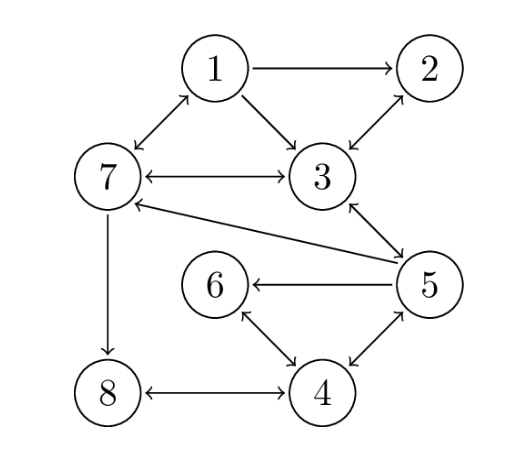
\includegraphics[width=0.5\textwidth]{web_graph2.png}
    \caption{Example web graph.}
    \label{fig:web_graph2}
\end{figure}

\noindent Research other references to the Google PageRank algorithm. After you complete your investigations, you will write a research paper. The tone of your paper is critical to us. Browse papers in the Astrophysical Journal or Physical Review to get a feel for the writing style that we are expecting. You will be submitting a single paper for your group. We have enclosed the LaTeX template that you have to use. Here is the outline of your paper:

\begin{itemize}
    \item Title
    \item Authors' Names
    \item Affiliation Name (The University of Texas at Austin)
    \item Abstract
    \item Keywords
    \item Introduction—In your introduction, you will research the background of this topic and summarize the importance of this algorithm in surfing the web. We want references to papers in published journals, not blogs on the Internet.
    \item You will state the algorithm and the code that you developed. 
    \item You will present and discuss your results.
    \item Conclusion - You will conclude by reflecting on how you can improve (if at all) the page rank of your website. You will discuss any future work you could have done by adding randomness to the algorithm Ex 4.100 (book) or EX 4.102 (online). 
    \item Acknowledgment - You will acknowledge any help from your classmates or the TAs.
    \item References
\end{itemize}

\section{Problem}

In this project you will discover how the Page Rank algorithm works to give the most relevant information as the top hit on a Google search.\\

\noindent Search engines compile large indexes of the dynamic information on the Internet so they are easily searched. This means that when you do a Google search, you are not actually searching the Internet; instead, you are searching the indexes at Google.\\

When you type a query into Google the following two steps take place:
\begin{enumerate}
    \item \textbf{Query Module}: The query module at Google converts your natural language into a language that the search system can understand and consults the various indexes at Google in order to answer the query. This is done to find the list of relevant pages. 
    \item \textbf{Ranking Module}: The ranking module takes the set of relevant pages and ranks them. The outcome of the ranking is an ordered list of web pages such that the pages near the top of the list are most likely to be what you desire from your search. This ranking is the same as assigning a popularity score to each web site and then listing the relevant sites by this score.
\end{enumerate}

\noindent This section focuses on the Linear Algebra behind the Ranking Module developed by the founders of Google: Sergey Brin and Larry Page. Their algorithm is called the Page Rank algorithm, and you use it every single time you use Googles (insert apostrophe) search engine.\\

\noindent In simple terms: A webpage is important if it is pointed to by other important pages.\\

\noindent The Internet can be viewed as a directed graph (look up this term here on Wikipedia) where the nodes are the web pages and the edges are the hyperlinks between the pages. The hyperlinks into a page are called in links, and the ones pointing out of a page are called out links. In essence, a hyperlink from my page to yours is my endorsement of your page. Thus, a page with more recommendations must be more important than a page with a few links. However, the status of the recommendation is also important.\\

\noindent Let us now translate this into mathematics. To help understand this we first consider the small web of six pages shown in Figure~\ref{fig:web_graph} (a graph of the router level of the internet can be found here). The links between the pages are shown by arrows. An arrow pointing into a node is an in link and an arrow pointing out of a node is an out link. In Figure~\ref{fig:web_graph}, node 3 has three out links (to nodes 1, 2, and 5) and 1 in link (from node 1).

\begin{figure}[H]
    \centering
    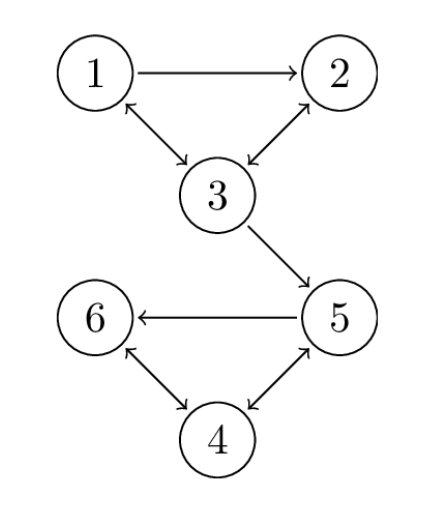
\includegraphics[width=0.4\textwidth]{web graph.png}
    \caption{Example web graph.}
    \label{fig:web_graph}
\end{figure}


\noindent We will first define some notation in the Page Rank algorithm:
\begin{itemize}
    \item $|P_i|$ is the number of out links from page $P_i$
    \item $\boldsymbol{H}$ is the \textit{hyperlink} matrix defined as:
        $$
            \boldsymbol{H}_{ij} =
            \begin{cases}
                \frac{1}{|P_j|}, & \text{if there is a link from node $j$ to node $i$} \\[6pt]
                0, & \text{otherwise}
            \end{cases}
        $$
    where the $i$ and $j$ are the row and column incides respectively.
    \item $\boldsymbol{x}$ is a vector that contains all of the Page Ranks for the individual pages.
\end{itemize}

\noindent The Page Rank algorithm works as follows:

\begin{enumerate}
    \item Initialize the page ranks to all be equal. This means that our initial assumption is that all pages are of equal rank. In the case of Figure~\ref{fig:web_graph} we would take $\boldsymbol{x}_0$ to be
        $$
            \boldsymbol{x}_0=
            \begin{pmatrix}
                1/6\\1/6\\1/6\\1/6\\1/6\\1/6
            \end{pmatrix}.
        $$
    \item Build the hyperlink matrix. As sn example, we'll consider node 3 in Figure~\ref{fig:web_graph}.
            There sre three out links from node 3 (to nodes 1, 2, and 5). Hence, $\boldsymbol{H}_{13}=1/3$, $\boldsymbol{H}_{23}=1/3$, and $\boldsymbol{H}_{53}=1/3$ 
            and the partially complete hyperlink matrix is
            $$\boldsymbol{H}=\begin{pmatrix}
                -&-&1/3&-&-&-\\
                -&-&1/3&-&-&-\\
                -&-&0&-&-&-\\
                -&-&0&-&-&-\\
                -&-&1/3&-&-&-\\
                -&-&0&-&-&-\\
            \end{pmatrix}
            $$
    \item The difference equation $\boldsymbol{X}_{n+1}=\boldsymbol{H}\boldsymbol{x}_n$ is used to iteratively refine the estimates of the page ranks. You can view the iterations as a person visiting a page and then following a link at random, then following a random link on the next page, and the next, and the next, etc. Hence we see that the iterations evolve exactly as expected for a difference equation.
            \begin{table}[H]
                \centering
                \begin{tabular}{|c|>{\raggedright\arraybackslash}p{6cm}|}
                \hline
                \textbf{Iteration} & \textbf{New Page Rank Estimation} \\
                \hline
                0 & $x_0$ \\
                1 & $x_1 = \boldsymbol{H} x_0$ \\
                2 & $x_2 = \boldsymbol{H} x_1 = \boldsymbol{H}^2 x_0$ \\
                3 & $x_3 = \boldsymbol{H} x_2 = \boldsymbol{H}^3 x_0$ \\
                4 & $x_4 = \boldsymbol{H} x_3 = \boldsymbol{H}^4 x_0$ \\
                $\vdots$ & $\vdots$ \\
                $k$ & $x_k = \boldsymbol{H}^k x_0$ \\
                \hline
                \end{tabular}
                % \caption{PageRank iterative computation}
            \end{table}
    \item When a steady state is reached we sort the resulting vector $\boldsymbol{x}_k$ to give the page rank. The node (web page) with the highest rank will be the top search result, the second highest rank will be the second search result, and so on.
            
\end{enumerate}

\noindent It doesn’t take much to see that this process can be very time consuming. Think about your typical web search with hundreds of thousands of hits; that makes a square matrix $\boldsymbol{H}$ 
that has a size of hundreds of thousands of entries by hundreds of thousands of entries! The matrix multiplications alone would take many minutes (or possibly many hours) for every search! …but Brin and Page were pretty smart dudes!!\\

\noindent We now state a few theorems and definitions that will help us simplify the iterative Page Rank process.


\section{Theorems}

\subsection*{Theorem 4.7}

If $\boldsymbol{A}$ is an $n\times n$ matrix with $n$ linearly dependent eigenvectors $\boldsymbol{v}_1,\boldsymbol{v}_2, \boldsymbol{v}_3,\cdots,\boldsymbol{v}_n$
and associated eigenvalues $\lambda_1,\lambda_2,\lambda_3,\cdots,\lambda_n$ then for any initial vector $\boldsymbol{x} \in \mathbb{R}^n$
we can write $\boldsymbol{A}^k\boldsymbol{x}$ as
$$
A^k\boldsymbol{x}=c_1\lambda_1^k\boldsymbol{v}_1+c_2\lambda_2^k\boldsymbol{v}_2+c_3\lambda_3^k\boldsymbol{v}_3+\cdots+c_n\lambda_n^k\boldsymbol{v}_n
$$

\noindent where $c_1,c_2,c_3,\cdots,c_n$ are the constants found by expressing $\boldsymbol{x}$ as a linear combination of the eigenvectors.\\

\noindent Note: We can assume that the eigenvalues are ordered such that $|\lambda_1|>|\lambda_2|\geq|\lambda_3|\geq\cdots\geq|\lambda_n|$.

\subsection*{Theorem 4.8}

A \textbf{probability vector} is a vector with entries on the interval $[0,1]$ that add up to 1.\\

\noindent A \textbf{stochastic matrix} is a square matrix whose columns are probability vectors.\\

\noindent If $\boldsymbol{A}$ is a stochastic $n\times n$ matrix then $\boldsymbol{A}$ will have $n$ linearly independent eigenvectors. Furthermore, the largest eigenvalue of a stochastic matrix will be
$\lambda_1=1$ and the smallest eigenvalue will always be nonnegative: $0\leq|\lambda_n|<1$.\


\subsection*{Theorem 4.9}

If $\boldsymbol{A}$ is an $n\times n$ stochastic matrix and $\boldsymbol{x}_0$  is some initial vector for the difference equation
$\boldsymbol{x}_{n+1}=\boldsymbol{A}\boldsymbol{x}_n$, then the steady state vector is
$$
\boldsymbol{x}_\text{equilibrium}=\lim_{k\to\infty}\boldsymbol{A}^k\boldsymbol{x}_0=?
$$

\noindent Proof:\\

\noindent First note that $\boldsymbol{A}$ is an $n\times n$ stochastic matrix so from Theorem 4.8. We know that there are $n$ linearly independent eigenvectors.
We can then substitute the eigenvalues from Theorem 4.8 in Theorem 4.7.
Noting that if $0<\lambda_j<1$ we have $\lim_{k\to\infty}\lambda_j^k=0$ the result follows immediately.

\section{Extra}

\subsection*{Exercise 4.102}

One thing that we didn’t consider in this version of the Google Page Rank algorithm is the random behavior of humans. One, admittedly slightly naive, modification that we can make to the present algorithm is to assume that the person surfing the web will randomly jump to any other page in the web at any time. For example, if someone is on page 1 in
Figure~\ref{fig:web_graph2} then they could randomly jump to any page 2 - 8. They also have links to pages 2, 3, and 7. That is a total of 10 possible next steps for the web surfer. There is a
$2/10$ chance of heading to page 2. One of those is following the link from page 1 to page 2 and the other is a random jump to page 2 without following the link. Similarly, there is a $2/10$ chance of heading to page 3, $2/10$ chance
of heading to page 7, and a $1/10$ chance of randomly heading to any other page.\\

\noindent Implement this new algorithm, called the random surfer algorithm, on the web in Figure~\ref{fig:web_graph2}.
Compare your ranking to the non-random surfer results from the previous problem.

\end{document}